\documentclass[a4paper]{article}

%use the english line for english reports
%usepackage[english]{babel}
\usepackage[portuguese]{babel}
\usepackage[utf8]{inputenc}
\usepackage{indentfirst}
\usepackage{graphicx}
\usepackage{verbatim}


\begin{document}

\setlength{\textwidth}{16cm}
\setlength{\textheight}{22cm}

\title{\Huge\textbf{Ploy}\linebreak\linebreak\linebreak
\Large\textbf{Relatório Final}\linebreak\linebreak
\linebreak\linebreak

\includegraphics[scale=0.1]{feup-logo.png}\linebreak\linebreak
\linebreak\linebreak
\Large{Mestrado Integrado em Engenharia Informática e Computação} \linebreak\linebreak
\Large{Programação em Lógica}\linebreak
}

\author{\textbf{Grupo CrazyPavement\_5:}\\ Gonçalo Ribeiro - 201403877 \\ Nuno Martins - 201405079 \\\linebreak\linebreak \\
 \\ Faculdade de Engenharia da Universidade do Porto \\ Rua Roberto Frias, s\/n, 4200-465 Porto, Portugal \linebreak\linebreak\linebreak
\linebreak\linebreak\vspace{1cm}}
\date{22 de Dezembro de 2016}
\maketitle
\thispagestyle{empty}

%************************************************************************************************
%************************************************************************************************

\newpage

\section*{Resumo}
Para o 2º Trabalho Prático, o nosso grupo implementou o puzzle "crazy pavement" em Prolog. O puzzle consiste em pintar grupos de células adjacentes em matrizes quadradas de forma a cumprir restrições arbitrárias, impostas sobre o número de células pintadas por linha ou por coluna. Foram empregues restrições lógicas ao nível do código. O resultado final é um gerador de soluções funcional, com interface de texto.

%Resumo sucinto do trabalho com 150 a 250 palavras (problema abordado, objetivo, como foi o problema resolvido/abordado, principais resultados e conclusões).

\newpage

\tableofcontents

%************************************************************************************************
%************************************************************************************************

%*************************************************************************************************
%************************************************************************************************

\newpage

%%%%%%%%%%%%%%%%%%%%%%%%%%
\section{Introdução}
No âmbito da unidade curricular de Programação em Lógica, foi-nos proposto para o segundo trabalho prático a elaboração de um puzzle em Prolog, recorrendo ao uso de restrições lógicas.

O objetivo deste trabalho foi pôr em prática os conhecimentos adquiridos sobre programação em lógica com restrições. Uma restrição lógica é uma limitação ao domínio de uma variàvel lógica. A linguagem Prolog pertence à classe de linguagens CLP - Contraint Logic Programming. Esta classe de linguagens combina a declaratividade da programação em lógica com a eficiência da resolução de restrições, substituindo o método de pesquisa predefinido da programação em lógica - "generate and test" - por "constrain and generate".

A problemática central do nosso trabalho reside na tradução das regras de um puzzle em restrições lógicas. Isto passa pela escolha de uma estrutura viável para a representação de soluções, e adaptar as regras linguísticas do puzzle em restrições do domínio lógico desta estrutura.

%%%%%%%%%%%%%%%%%%%%%%%%%%
\section{O Jogo Ploy}
Ploy é um jogo de tabuleiro para 2 ou 4 jogadores. Neste trabalho apenas nos focámos na versão de 2 jogadores.

Lançado em 1970 pela a empresa Minnesota Mining and Manufacturing, o jogo consiste num tabuleiro 9 por 9 onde cada jogador tem um conjunto de 15 peças.
O objetivo do jogo é capturar o Commander adversário (semelhante ao Rei no xadrez) ou então todas as peças menos o Commander. A captura de peças efectua-se da mesma maneira que no xadrez - movendo-se um peça para uma casa ocupada por uma peça adversária.

Em cada turno, o jogador pode escolher uma peça para jogar. Uma jogada consiste em rodar a peça escolhida (45º para qualquer sentido) ou então mover a peça numa das direções para qual ela aponta. O número de casas a mover é determinado pelo tipo de peça.

Cada conjunto de peças contem:

\begin{table}[ht]
\centering
%\label{Conjunto de peças de cada jogador.}
\begin{tabular}[ht]{|c|c|c|c|c|}
  \hline
Propriedades \textbackslash \space Peças&Shields(*)&Probes&Lances&Commander\\
\hline
Quantidade&3&5&6&1\\
Casas a mover&1&2&3&1\\
Direções apontadas&1&2&3&4\\
\hline
\end{tabular}
\caption{(*) Os Shields são as únicas peças que podem ser rodadas e movidas na mesma jogada.}
\end{table}

\begin{figure}[ht]
\caption{Estado inicial do jogo.}
\centering
\includegraphics[scale=0.8]{ploy.PNG}
\end{figure}
%%%%%%%%%%%%%%%%%%%%%%%%%%
\section{Lógica do Jogo}

%Descrever o projeto e implementação da lógica do jogo em Prolog, incluindo a forma de representação do estado do tabuleiro e sua visualização, execução de movimentos, verificação do cumprimento das regras do jogo, determinação do final do jogo e cálculo das jogadas a realizar pelo computador utilizando diversos níveis de jogo. Sugere-se a estruturação desta secção da seguinte forma:

\subsection{Representação do Estado do Jogo}
O jogo é representado por uma lista. Dentro desta lista, existem 9 listas que representam as 9 linhas do tabuleiro. Dentro de cada uma destas últimas, 9 listas adicionais que representam as 9 quadriculas de cada linha. Dentro de cada quadricula, existe o nome da equipa ocupante - 'red', 'green' ou 'empty', caso esteja desocupada - e uma lista de pontos cardeais para qual a peça ocupante aponta (esta lista é vazia caso não exista peça).

Exemplo da estrutura do jogo:
\begin{verbatim}
%%%%%%%%%%%%%%%%%%%%%%%
%% Tabuleiro de jogo %%
%%%%%%%%%%%%%%%%%%%%%%%
board(
[
[*casa*,*casa*,*casa*,*casa*,*casa*,*casa*,*casa*,*casa*,*casa*],
[*casa*,*casa*,*casa*,*casa*,*casa*,*casa*,*casa*,*casa*,*casa*],
[*casa*,*casa*,*casa*,*casa*,*casa*,*casa*,*casa*,*casa*,*casa*],
[*casa*,*casa*,*casa*,*casa*,*casa*,*casa*,*casa*,*casa*,*casa*],
[*casa*,*casa*,*casa*,*casa*,*casa*,*casa*,*casa*,*casa*,*casa*],
[*casa*,*casa*,*casa*,*casa*,*casa*,*casa*,*casa*,*casa*,*casa*],
[*casa*,*casa*,*casa*,*casa*,*casa*,*casa*,*casa*,*casa*,*casa*],
[*casa*,*casa*,*casa*,*casa*,*casa*,*casa*,*casa*,*casa*,*casa*],
[*casa*,*casa*,*casa*,*casa*,*casa*,*casa*,*casa*,*casa*,*casa*]
]
).
\end{verbatim}

Exemplo da estrutura de uma *casa*:
\begin{verbatim}
%%%%%%%%%%%%%%%%%%%%%%
%% Quadricula vazia %%
%%%%%%%%%%%%%%%%%%%%%%
['empty',[]]

%%%%%%%%%%%%%%%%%%%%%
%% Commander verde %%
%%%%%%%%%%%%%%%%%%%%%
['green',['sw','se','ne','nw']]
\end{verbatim}



\subsection{Visualização do Tabuleiro}% (Pode ser idêntico ao descrito no relatório intercalar.)
A visualização do tabuleiro é feita através do predicado \textit{draw\_board(Tab)}. Neste predicado, Tab representa a estrutura de jogo supracitada - uma lista de listas. O predicado escreve a representação ASCII do tabuleiro no output buffer da consola em questão. Cada peça é representada no centro com o caracter inicial da cor correspondente (Red ou Green) e também com os respectivos indicadores de direção.

\begin{figure}[ht]
\caption{Representação do jogo em ASCII.}
\centering
\includegraphics[scale=0.8]{tabuleiro.png}
\end{figure}

\subsection{Execução de Jogadas}% Validação e execução de uma jogada num tabuleiro, obtendo o novo estado do jogo. Exemplo: \textit{move(+Move, +Board, -NewBoard)}.
A realização de jogadas é feita através dos predicados:

\begin{itemize}
  \item \textit{movePiece(+X,+Y,+Orientation,+Length,+Board,-NewBoard,-Consumed)}
  \item \textit{rotatePiece(+Piece,+Orientation,-PieceNova)}
  \item \textit{setPiece(+X,+Y,+Board,-NewBoard,-NewPiece)}
\end{itemize}

Estes predicados retornam todos novo estado de jogo - NewBoard.

O predicado \textit{movePiece} também retorna o número de direções da peça consumida (0 se nao foi consumida nenhuma), o que permite identificar o tipo de peça capturada.
Neste predicado, são efetuadas várias verificações quanto à possibilidade de movimento da peça, nomeadamente:
\begin{itemize}
  \item Se a Orientation está presente na peça - \textit{assertHasOrientation(Orientation,Piece)};
  \item Se a distância é possível - \textit{assertValidLength(Length,Piece)};
  \item Se o destino está dentro do tabuleiro - \textit{assertInsideBoundaries(Xf,Yf)};
  \item Se todas as casas até ao destino estão vazias, e se o destino ou está vazio ou contem um inimigo - \textit{assertNoCollision(X,Y,Orientation,Length,Board)}.
\end{itemize}

A rotação de uma peça é efetuada através de \textit{rotatePiece} e \textit{setPiece}, não sendo necessárias nenhumas verificações, pois a rotação de uma peça nunca pode falhar.

\subsection{Final do Jogo}
%Verificação do fim do jogo, com identificação do vencedor. Exemplo: \textit{game\_over(+Board, -Winner)}.
O predicado \textit{assertGameEnded(+Board,-Winner)} faz a  verificação do final do jogo.
Neste predicado, Board representa o estado de jogo atual, e Winner refere a equipa vitoriosa caso o predicado seja verdadeiro.

Por sua vez , este predicado chamará outros 2 predicados para cada equipa, \textit{assertCommanderDead(+Board,+Team)} e \textit{assertAllSmallDead(+Board,+Team)}, que testam as duas condições de terminação de jogo, que são, respetivamente, quando o Commander de uma das equipas é capturado ou quando todas as peças excepto o Commander de uma equipa são capturadas.

\subsection{Jogada do Computador}% Escolha da jogada a efetuar pelo computador, dependendo do nível de dificuldade. Por exemplo: \textit{choose\_move(+Level, +Board, -Move)}.
O predicado \textit{bot\_plays\_diff(Dif,Board,Team,NewBoard)} faz uma jogada automática.
Neste predicado, Dif representa a dificuldade do bot, Board é o estado de jogo atual, Team a equipa do bot e NewBoard o novo estado de jogo depois de efetuada a jogada. Dif pode tomar 2 valores possíveis, podendo estes ser 0 (bot aleatório) e 1 (bot ganancioso).

O bot aleatório fará sempre jogadas completamente aleatórias, enquanto que o bot ganancioso procurará recursivamente qual a melhor jogada a fazer nesse mesmo turno, sendo o factor a maximizar a peça inimiga capturada(quantas mais direçoes tiver a peça, maior a prioridade). Assim, uma peça com 4 direções tem prioridade sobre uma de 3, esta tem prioridade sobre uma de 2, e a de 2 tem prioridade sobre a de 1.

Se não for encontrada nenhuma jogada que resulte na captura de uma peça, o bot ganancioso chama o predicado do bot aleatório, ou seja, com Dif = 0.

%%%%%%%%%%%%%%%%%%%%%%%%%%
\section{Interface com o Utilizador}
%Descrever o módulo de interface com o utilizador em modo de texto.
Ao correr o programa, o utilizador é deparado com o menu principal.

\begin{figure}
\caption{Menu principal.}
\centering
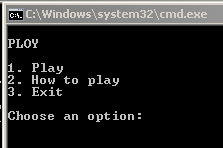
\includegraphics[scale=1]{menu.png}
\end{figure}

O menu tem três opções: 'Play', 'How to play' e 'Exit'.

A opção 'Play' imprime os modos de jogo disponiveis.

\begin{figure}
\caption{Menu 'Play'.}
\centering
\includegraphics[scale=1]{play.png}
\end{figure}

Uma vez escolhido um modo de jogo onde o utilizador intervine (Player Vs. Player e Player Vs. AI), o utilizador terá a opção de fazer uma jogada.
A jogada é constituida pela escolha de uma peça, seguida pela escolha entre mover ou rodar essa peça (ou ambas caso a peça seja um Shield).

\begin{figure}
\caption{Um turno do jogador vermelho (\textit{input} em baixo).}
\centering
\includegraphics[scale=0.65]{jogada.png}
\end{figure}

\begin{figure}
\caption{Turno do jogador verde.}
\centering
\includegraphics[scale=0.65]{pos_jogada.png}
\end{figure}

A opção 'How to play' imprime as instruções do jogo no ecrã e remete novamente para o menu inicial.

\begin{figure}
\caption{Manu 'How to play'.}
\centering
\includegraphics[scale=0.7]{how.png}
\end{figure}



%%%%%%%%%%%%%%%%%%%%%%%%%%
\section{Conclusões}
Como considerações finais, estamos satisfeitos com o trabalho que realizámos e concordamos que foi uma experiência enriquecedora e que de certa forma colocou à prova os nossos conhecimentos de lógica.

De momento, todos os puzzles são hardcoded. Reconhecemos que a implementação de uma funcionalidade que permitisse ao utilizador ler puzzles a partir de ficheiros sería uma melhoria conveniente, assim como a adição de um menu "how to play" para orientar novos utilizadores ao funcionamento do programa.

Visto que o cerne do nosso código - o predicado que gera soluções do puzzle - foi desenvolvido numa única aula prática, reconhecemos o poder da programação com restrições lógicas na resolução deste tipo de problemas combinatórios. É de nossa opinião que a mesma implementação num paradigma de linguagem imperativo (C, Java, etc.) resultaria num tempo desenvolvimento maior e num código mais extenso e complexo.

%Que conclui deste projecto? Como poderia melhorar o trabalho desenvolvido?
\end{document}
